\documentclass{setup}

\assignment{Initial idea: Visual Question Answering}
\authorOne{Jorrit Willaert} 
\studentnumberOne{r0652971} 

\begin{document}
	\maketitle

	DeepProbLog offers the ability to integrate probabilistic knowledge with deep neural networks. This way, the strength of neural networks (system 1: typical subconscious tasks such as visual recognition, the processing of languages, \dots) is complemented with the strength of rule-based mechanisms (system 2: slow, sequential thinking such as the derivation of a proof). I propose an application that requires the integration of both systems.

	The Sort-of-CLEVR dataset is a simplified version of the CLEVR dataset \cite{clevr_dataset}. This simplified dataset is composed of 10 000 images with per image 20 accompanied questions. An image consists of spread out objects, with randomly chosen shapes and colors. The questions are divided in two categories: non-relational and relational questions. Non-relational questions ask for example about the shape, the horizontal or vertical location of the colored object. Relational questions, on the other hand, ask about the shape of the object which is closest (or furthest) to a certain colored object, or ask about the number of objects with the same shape \cite{sort_of_clevr_dataset}.

	\begin{figure}[htbp]
		\centerline{\fbox{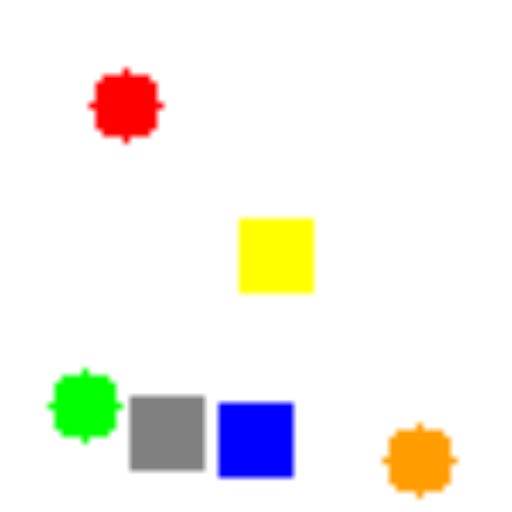
\includegraphics[scale=.25]{example_image_of_dataset.png}}}
		\caption{A sample image from the Sort-of-CLEVR dataset \cite{sort_of_clevr_dataset}}
		\label{image:example_image_of_dataset}
		\end{figure}

	A sample image is given in Figure \ref{image:example_image_of_dataset}. With this sample image, an answer on a non-relational question such as "What is the shape of the blue object?" would be: "square", while an answer on a relational question such as "How many objects have the same shape as the blue one?" would be: "3".

	I propose to generate data based on the Sort-of-CLEVR dataset, with the simplification that objects may not be entirely randomly located, but instead only in certain positions on a grid. A 5 by 5 grid could for example be used. The generation of new images and accompanied questions is rather straightforward, which could probably even be done at training time.
	
	I would use 25 convolutional neural networks, one for each grid position. The output would naturally be if an object is located in that position, and what its shape and color is. Once the location, shapes and colors of the objects are known, rule-based mechanisms can be used to answer the accompanied questions.

	\bibliographystyle{plain} 
	\bibliography{Capita_Selecta_AI_Initial_Idea} 
	
\end{document}